\chapter{Medotologia}\label{cap:CnptDsng}
\section{ARDUINO RTU}
\section{ARDUINO ETHERNET TCP}
\section{Elipse RTU}
\section{Elipse TCP}
\section{Interface Gráfica}

\section{Escolha da frequência}\label{sec:esc_freq}
A frequência foi escolhida com base no regulamento da Anatel. O mesmo estabelece que equipamentos de radiocomunicação com faixas restritas de: 902-907,5; 915-928; 2400-2483,5; 5725-5850 MHz, assim para os cálculos iniciais foi escolhida uma frequência de 920MHz.

\section{Estudo do Obstáculo}\label{sec:est_obs}
O primeiro passado adotado foi a análise dos pontos, verificando se entre os dois existia algum obstáculo. Essa informação pode ser extraída dos mapas que foram fornecidos em anexo, como mostra a figura \ref{fig:obs_cam}.
\begin{figure}[h]
	\centering
	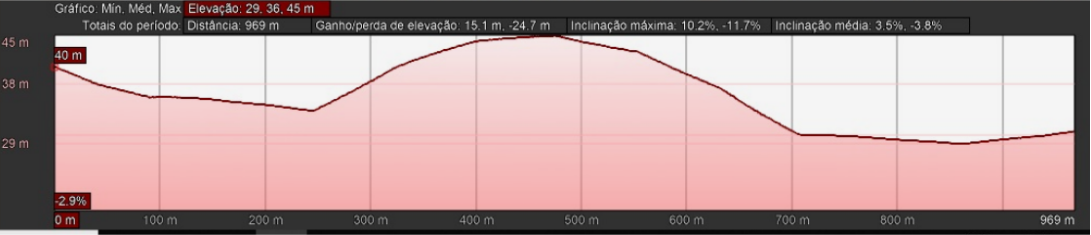
\includegraphics[width=1\textwidth]{obs_cam.png}
	\caption{Gráfico de obstáculo}
	\label{fig:obs_cam}
	%\source{Fornecido junto com os pontos}
\end{figure} 

Por meio da análise do gráfico, fica evidenciado que entre os dois pontos existe um grande obstáculo arredondado, assim sendo necessário calcular o seu raio de curvatura e a partir disso ver o quanto ele irá interferir na transmissão.
É feita uma aproximação do topo do obstáculo, utilizando uma curvatura parabólica como mostrado na figura 4 \ref{fig:obs_raio}.
\begin{figure}[h]
	\centering
	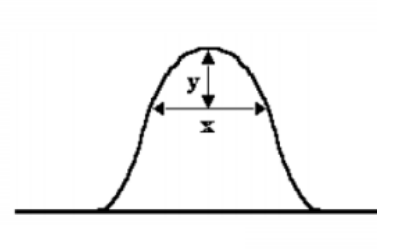
\includegraphics[width=.4\textwidth]{obs_raio.png}
	\label{fig:obs_raio}
	\caption{Curvatura parabólica utilizada para aproximação}
	%\source{Própria}
\end{figure} 



